
\begin{figure}[h!tb]\begin{center}
	\subfigure[]{
  	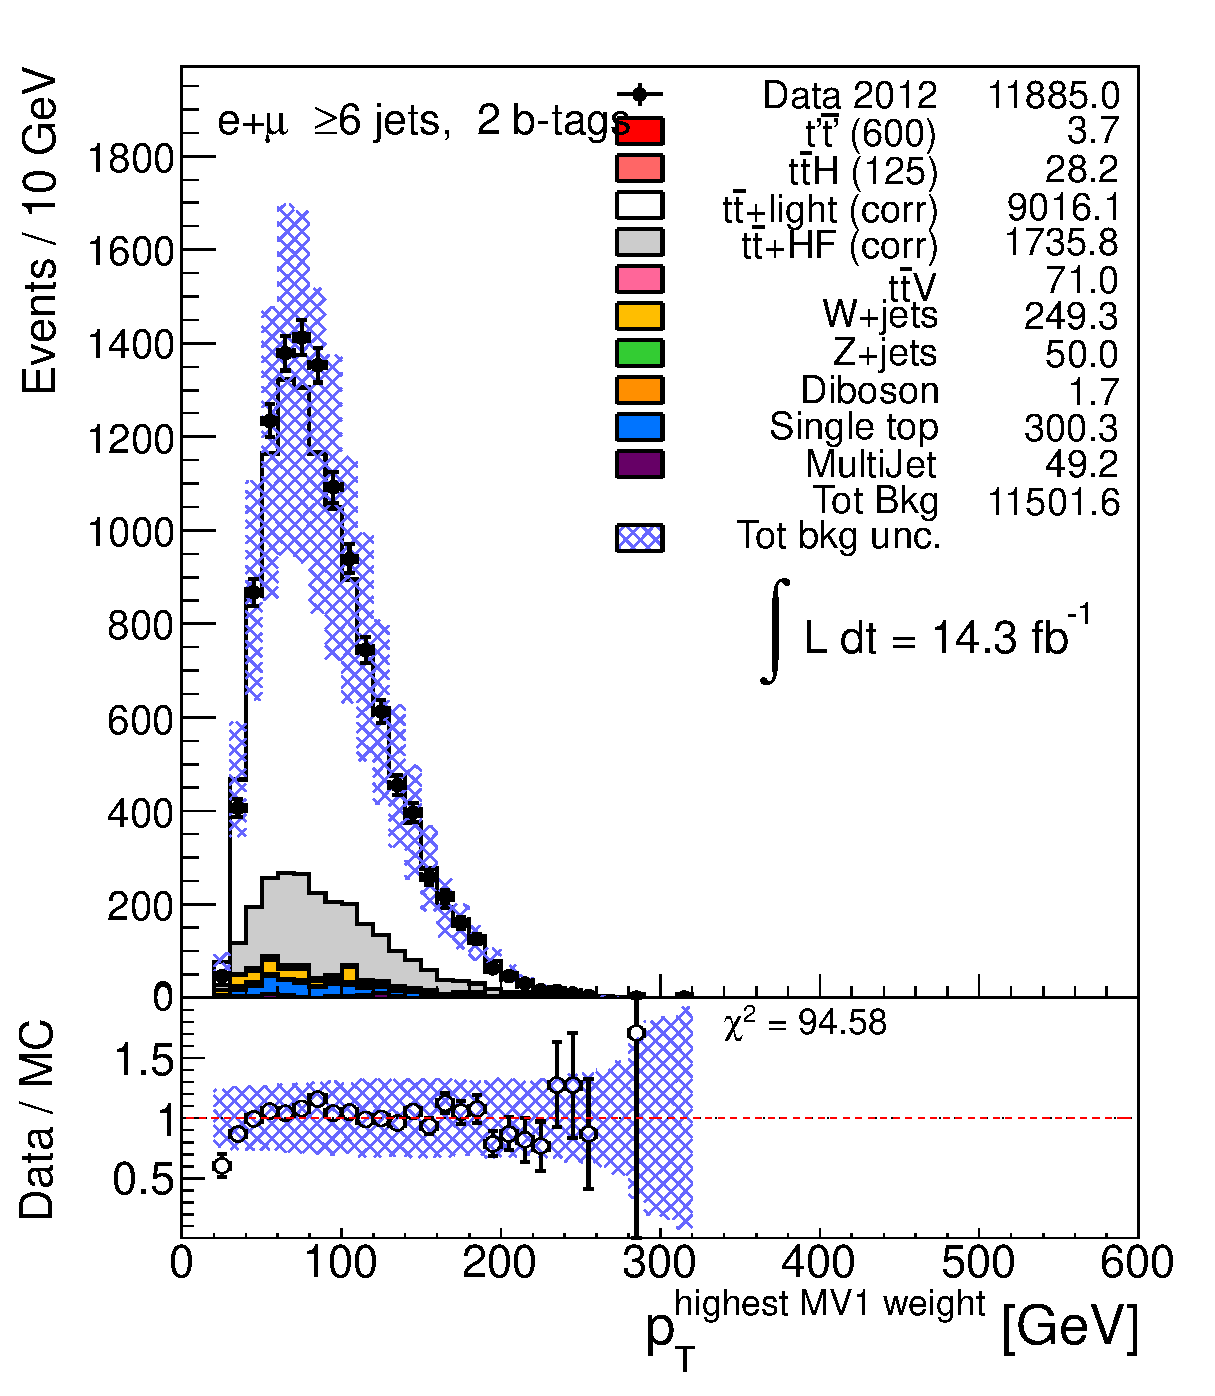
\includegraphics[width=0.235\textwidth]{htx_analysis_14ifb/figures/scaled_cr_blind/JetPtB1_ELEMUON_6jetin2btagex_NOMINAL}}
	\subfigure[]{
  	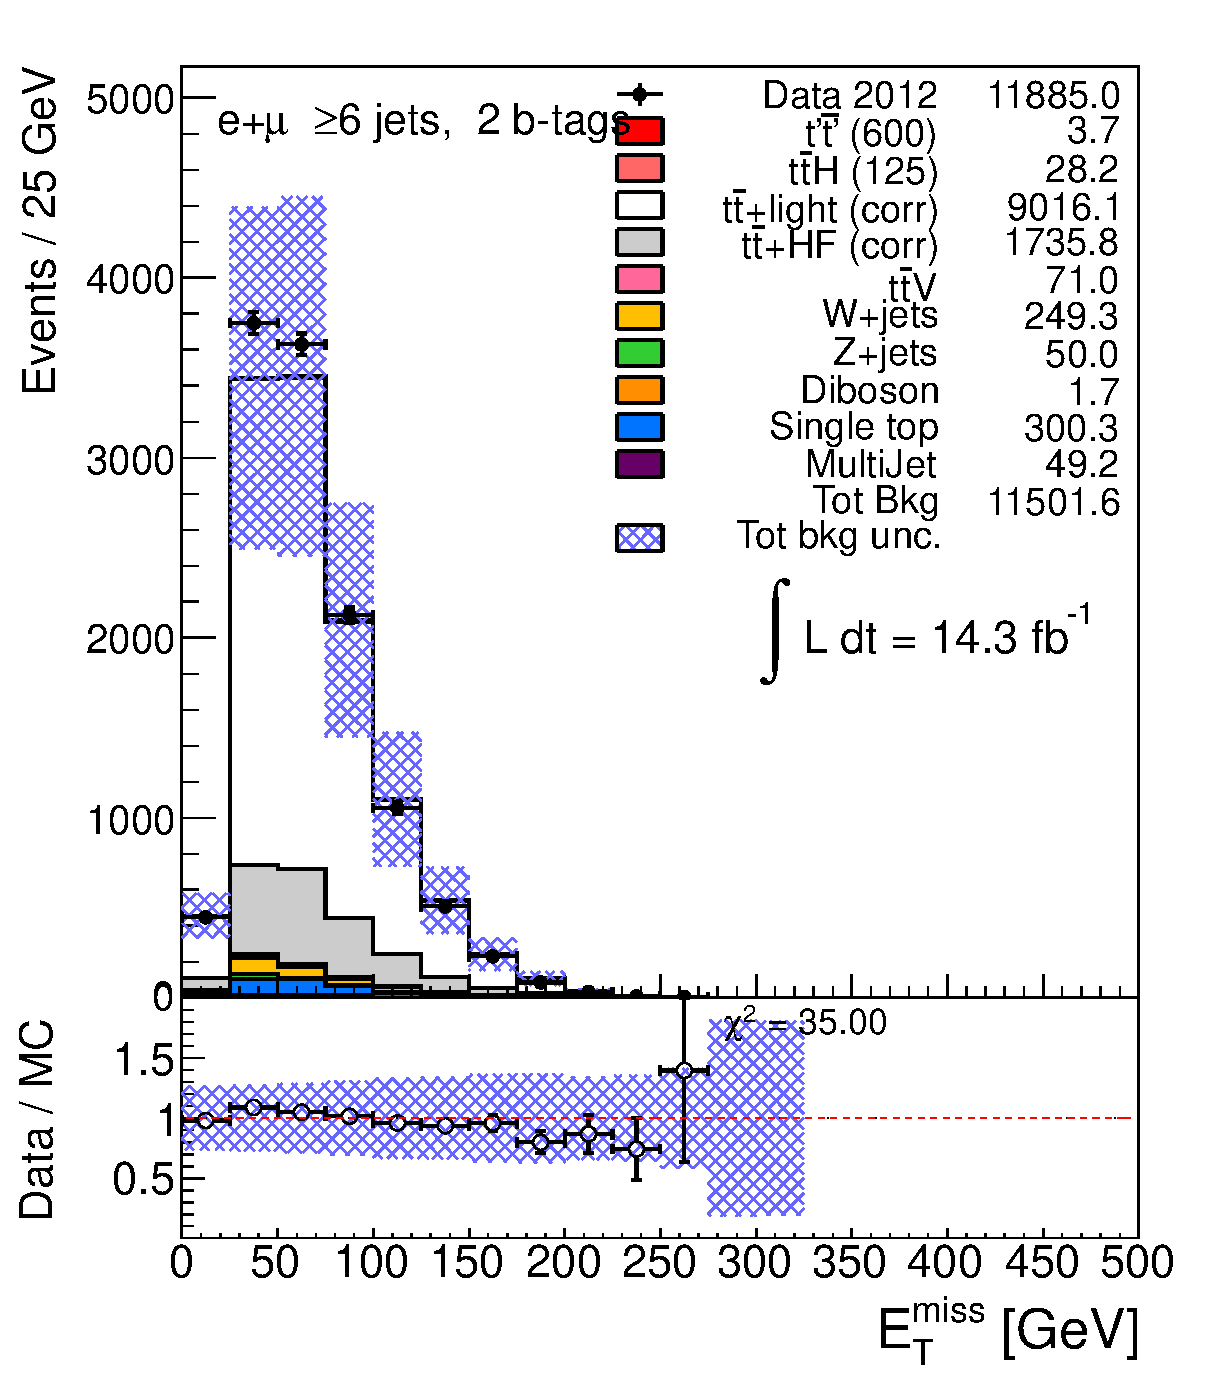
\includegraphics[width=0.235\textwidth]{htx_analysis_14ifb/figures/scaled_cr_blind/MET_ELEMUON_6jetin2btagex_NOMINAL}}
	\subfigure[]{
  	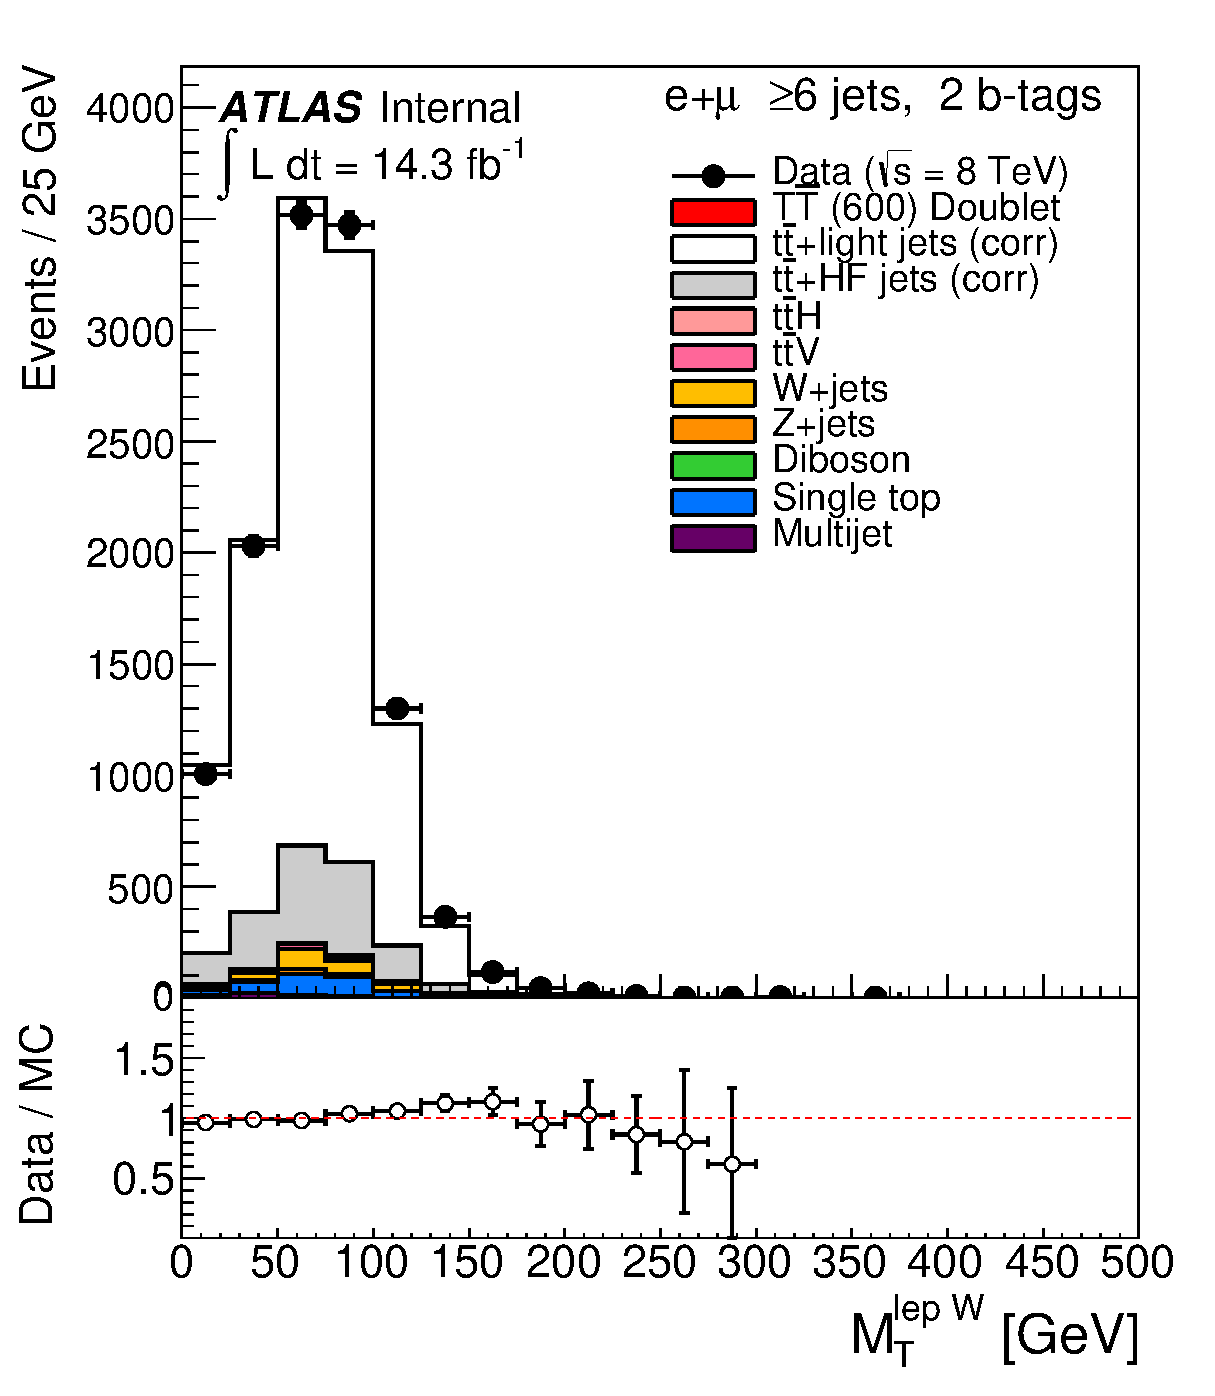
\includegraphics[width=0.235\textwidth]{htx_analysis_14ifb/figures/scaled_cr_blind/Wlep_MassT_ELEMUON_6jetin2btagex_NOMINAL}}
	\subfigure[]{
  	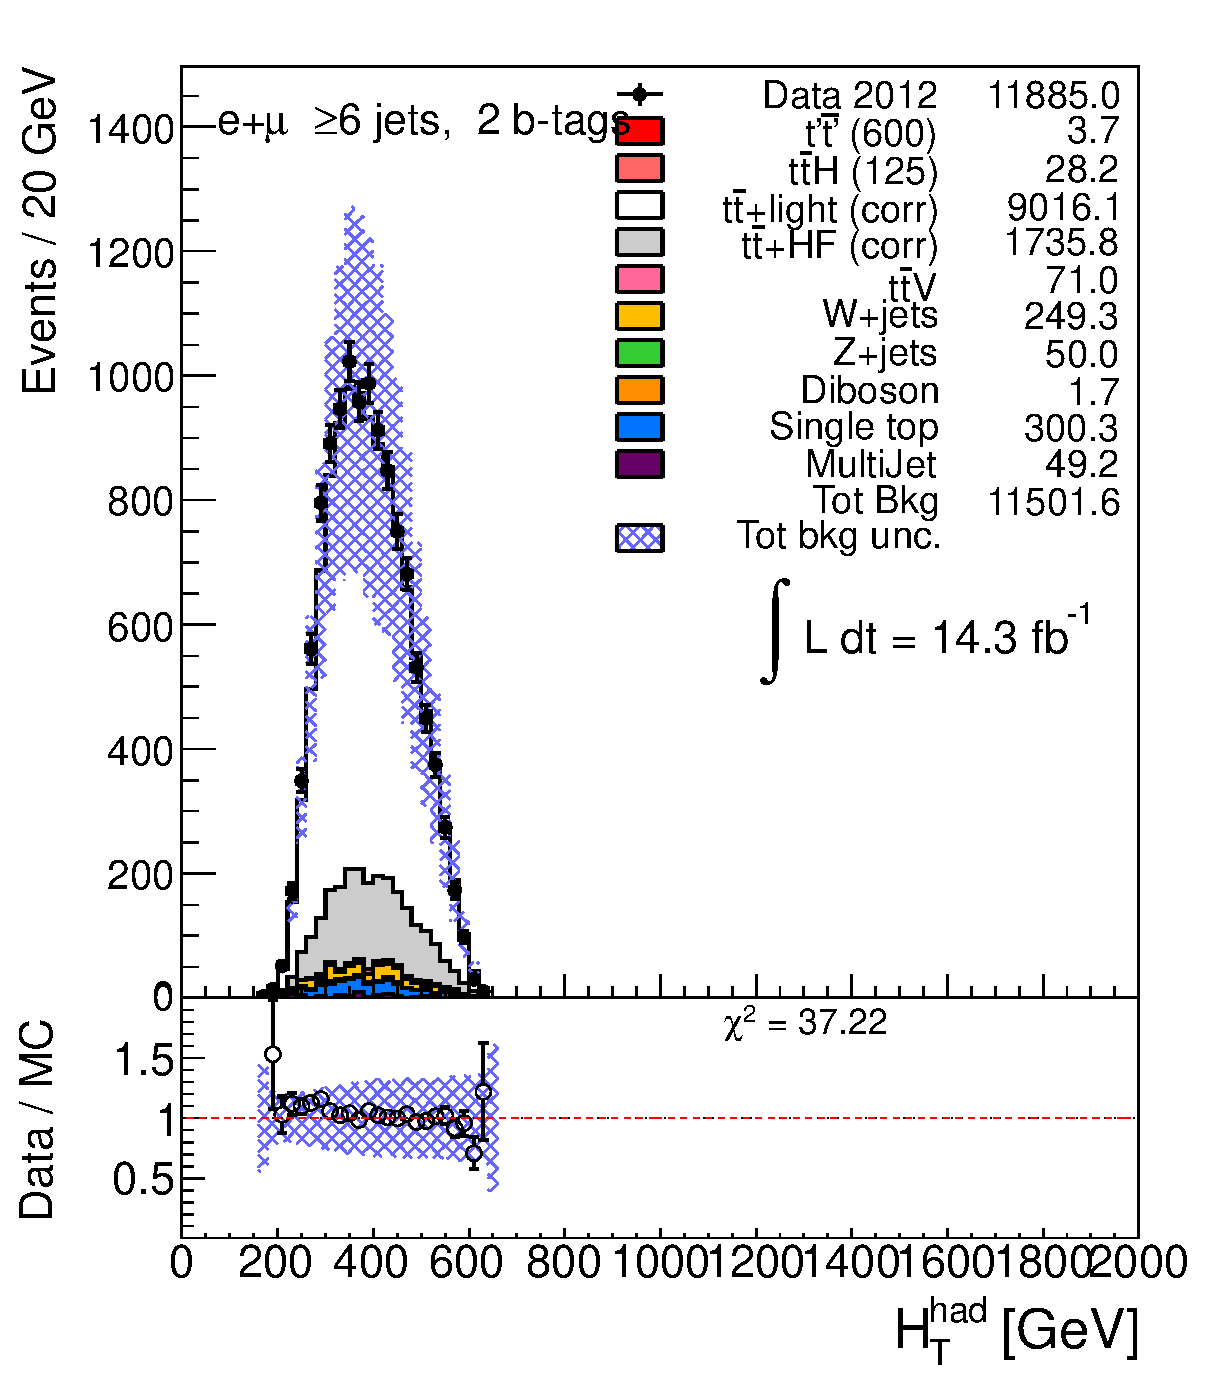
\includegraphics[width=0.235\textwidth]{htx_analysis_14ifb/figures/scaled_cr_blind/HTHad_ELEMUON_6jetin2btagex_NOMINAL}}\\
	\subfigure[]{
  	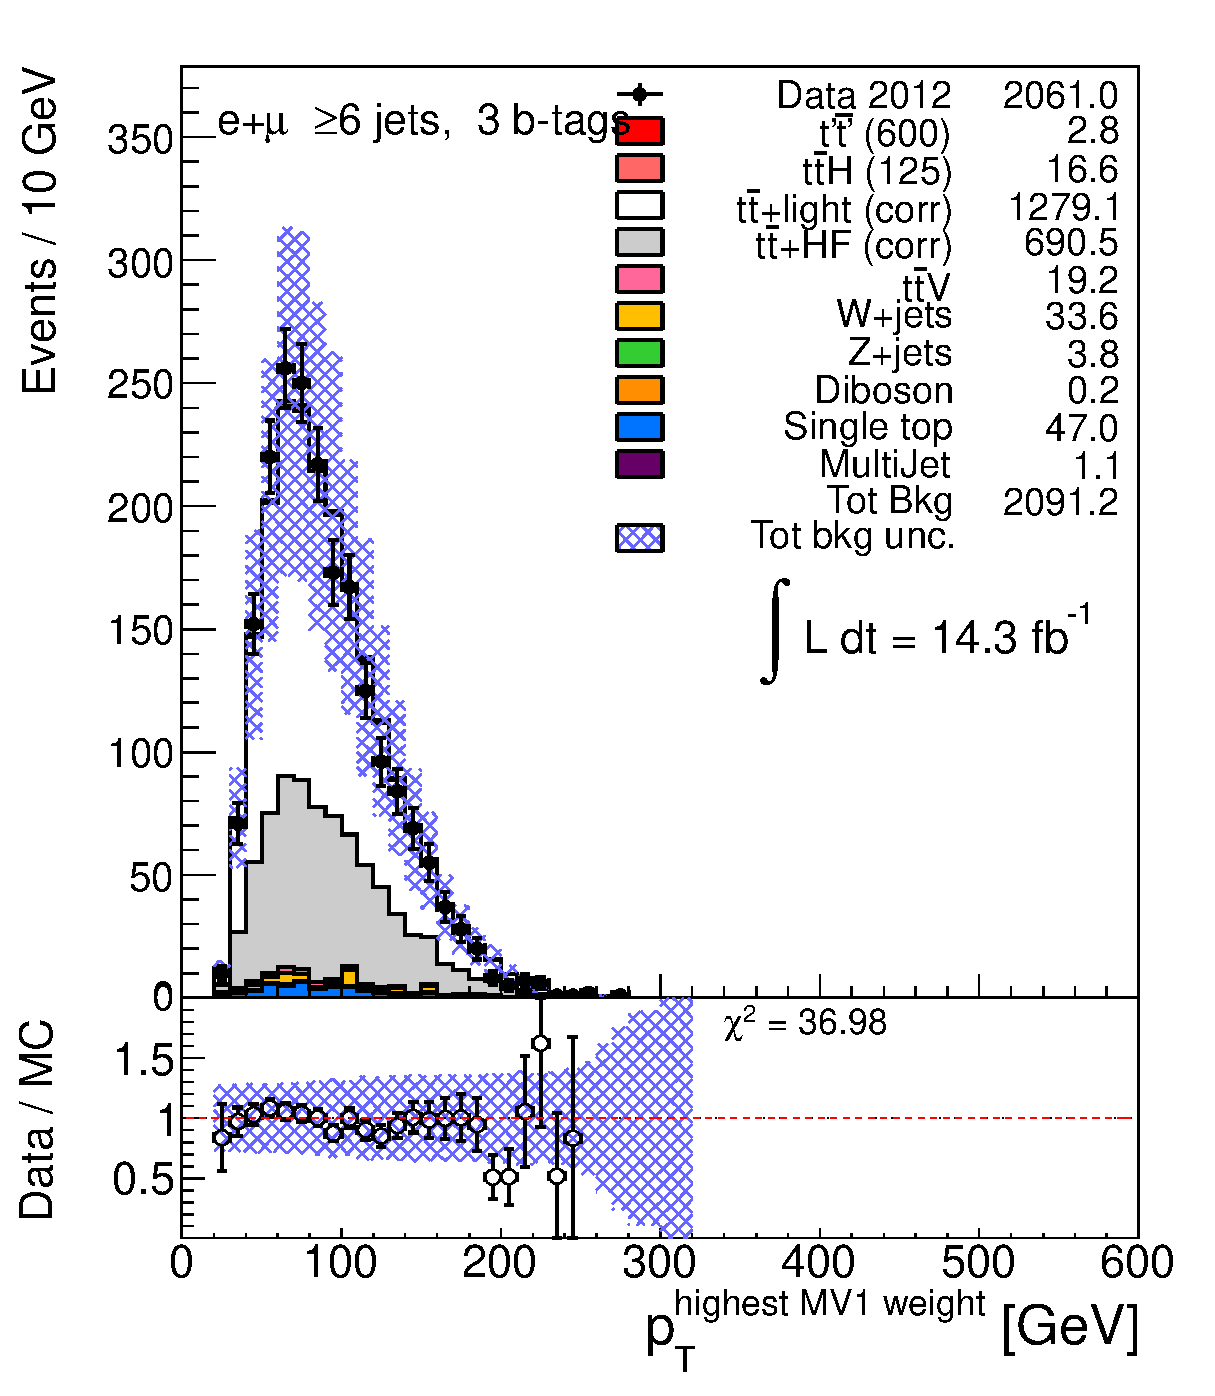
\includegraphics[width=0.235\textwidth]{htx_analysis_14ifb/figures/scaled_cr_blind/JetPtB1_ELEMUON_6jetin3btagex_NOMINAL}}
	\subfigure[]{
  	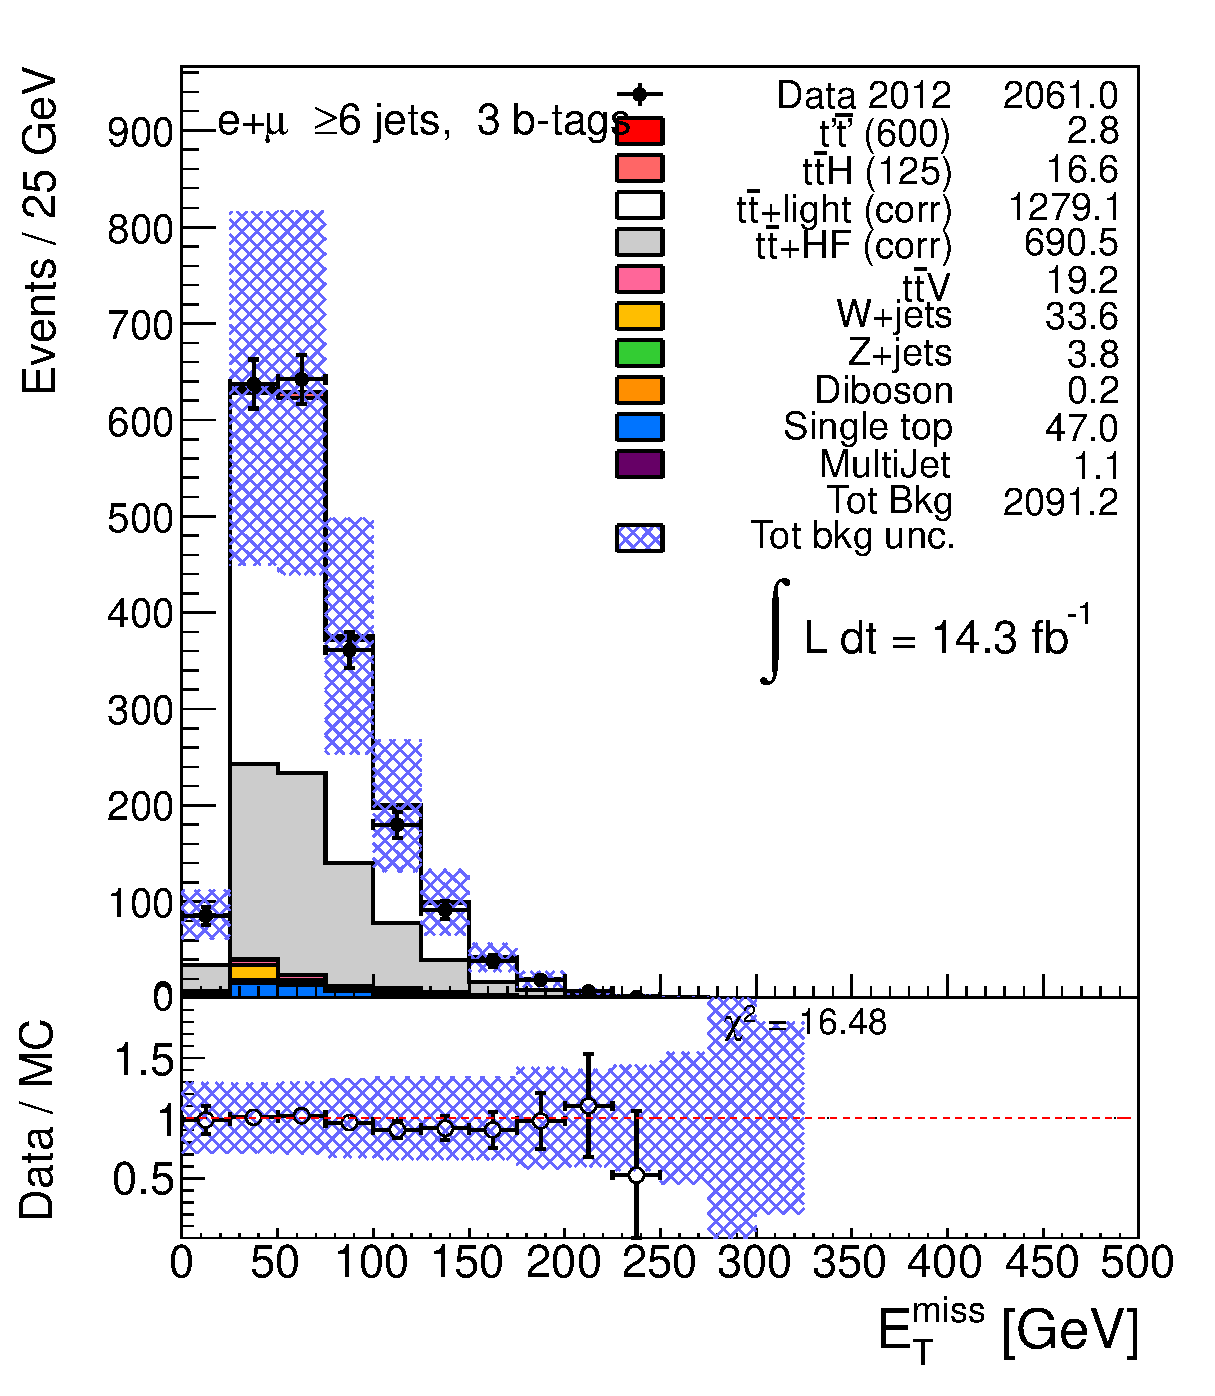
\includegraphics[width=0.235\textwidth]{htx_analysis_14ifb/figures/scaled_cr_blind/MET_ELEMUON_6jetin3btagex_NOMINAL}}
	\subfigure[]{
  	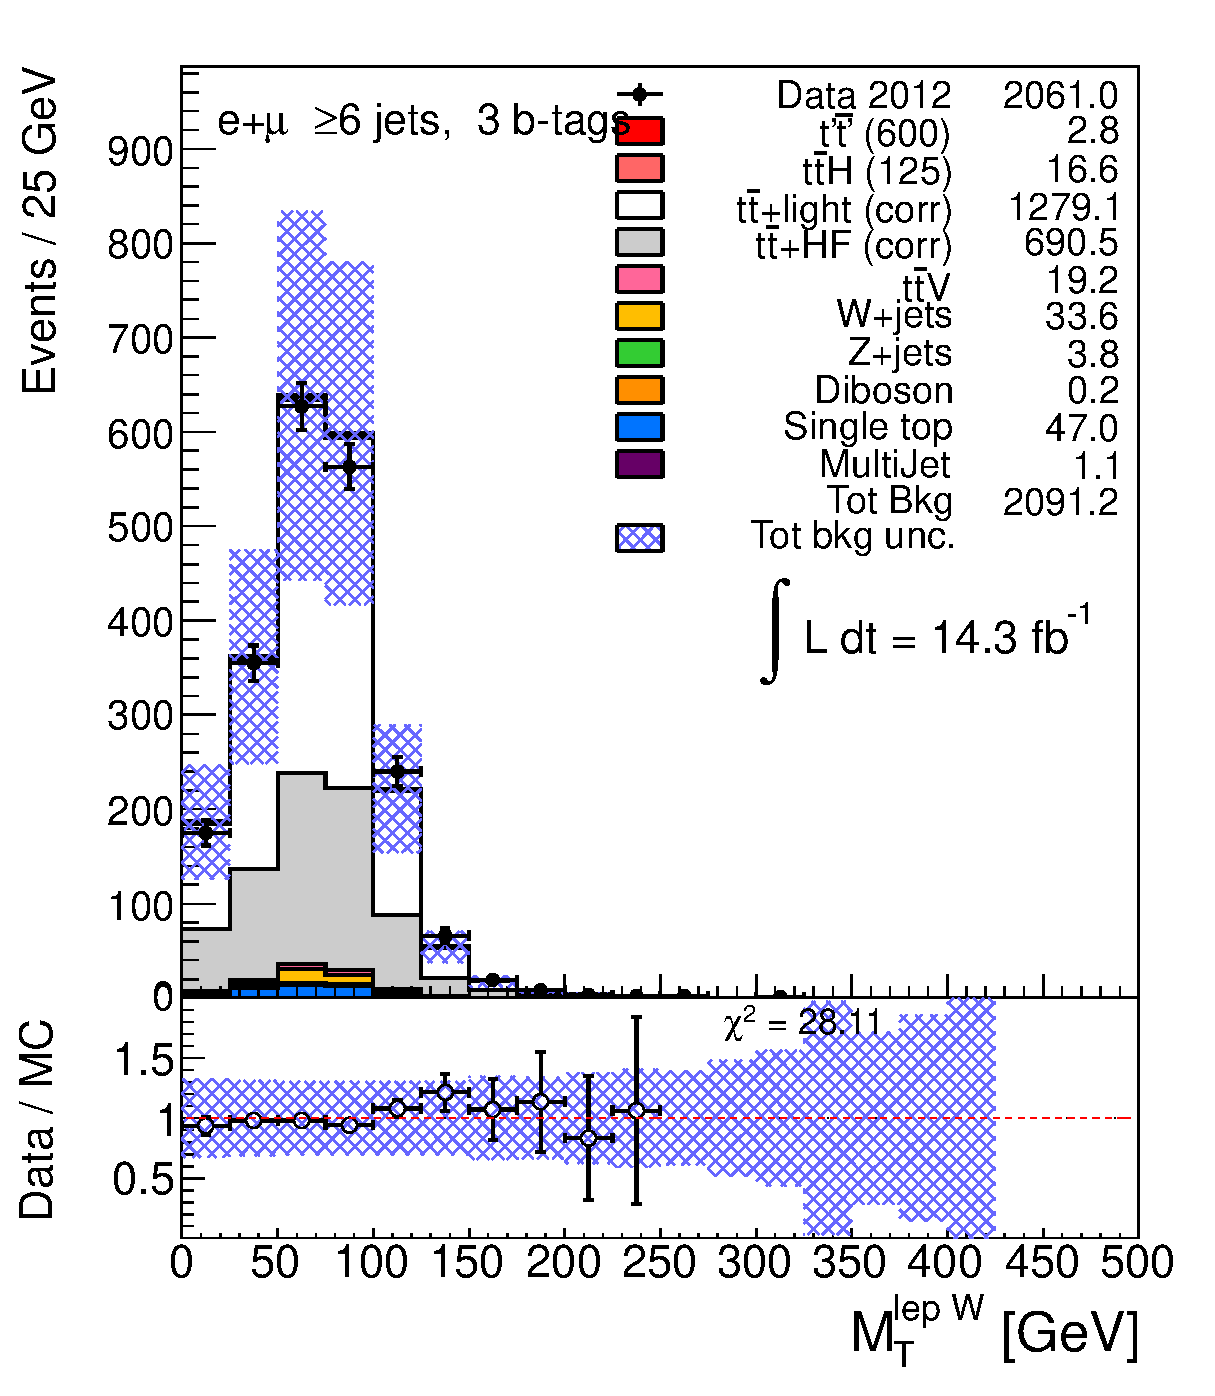
\includegraphics[width=0.235\textwidth]{htx_analysis_14ifb/figures/scaled_cr_blind/Wlep_MassT_ELEMUON_6jetin3btagex_NOMINAL}}
	\subfigure[]{
  	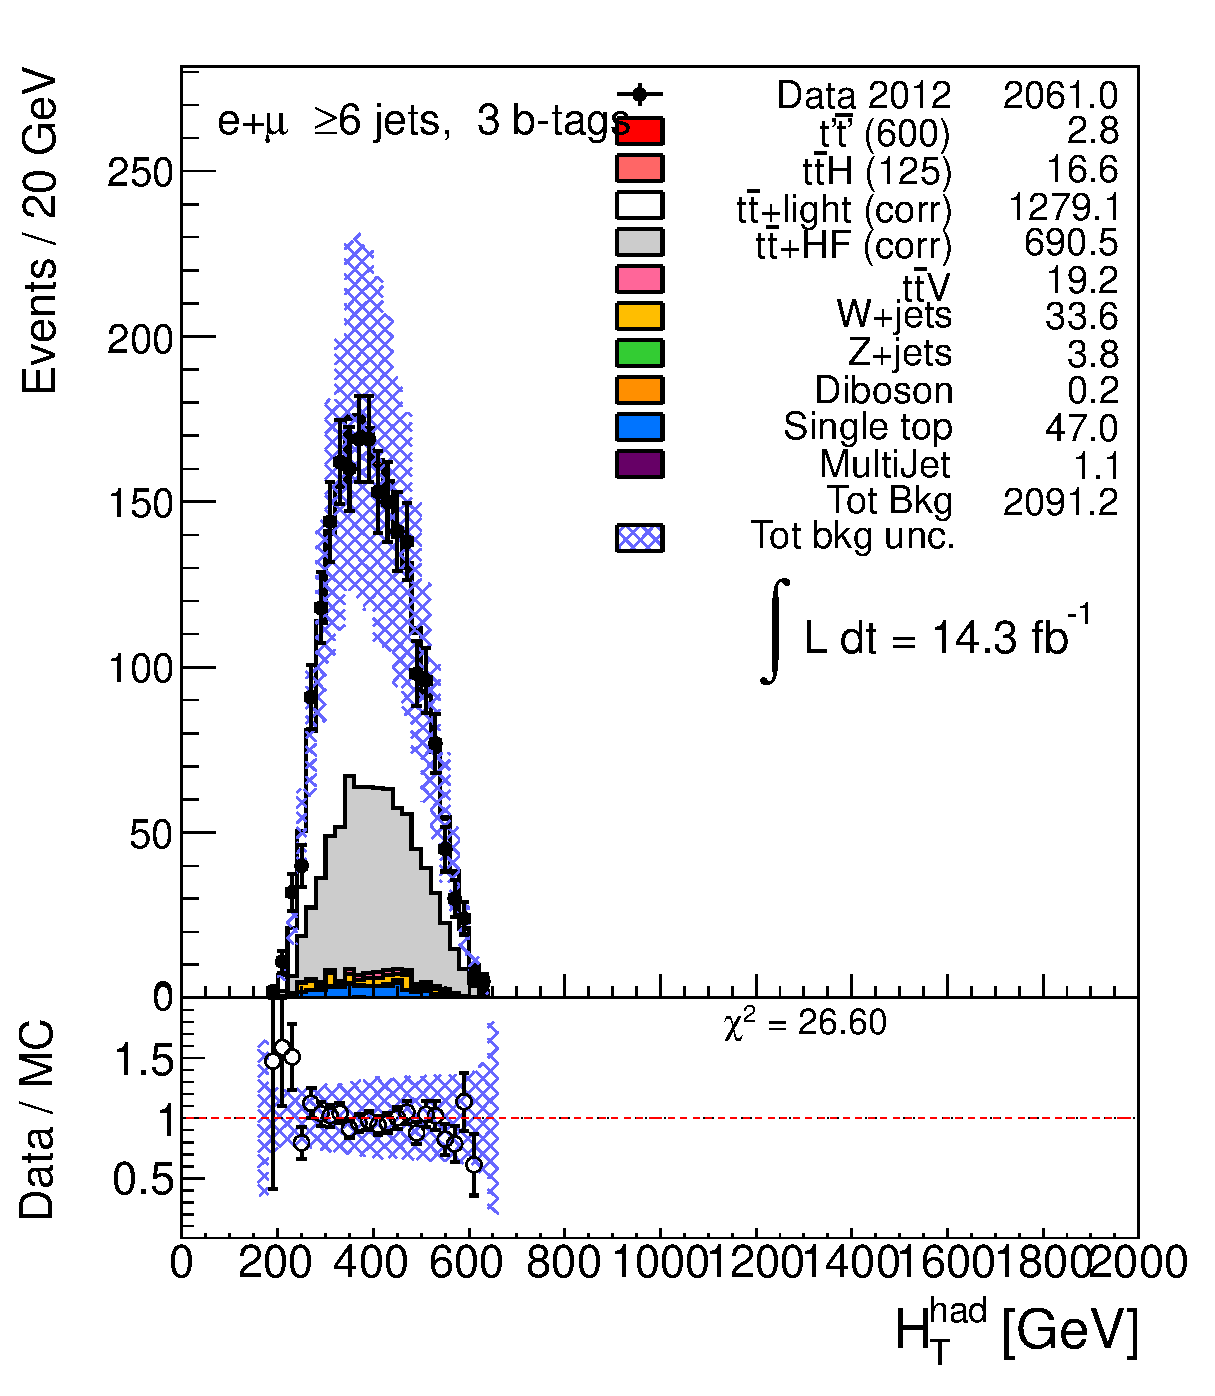
\includegraphics[width=0.235\textwidth]{htx_analysis_14ifb/figures/scaled_cr_blind/HTHad_ELEMUON_6jetin3btagex_NOMINAL}}\\
	\subfigure[]{
  	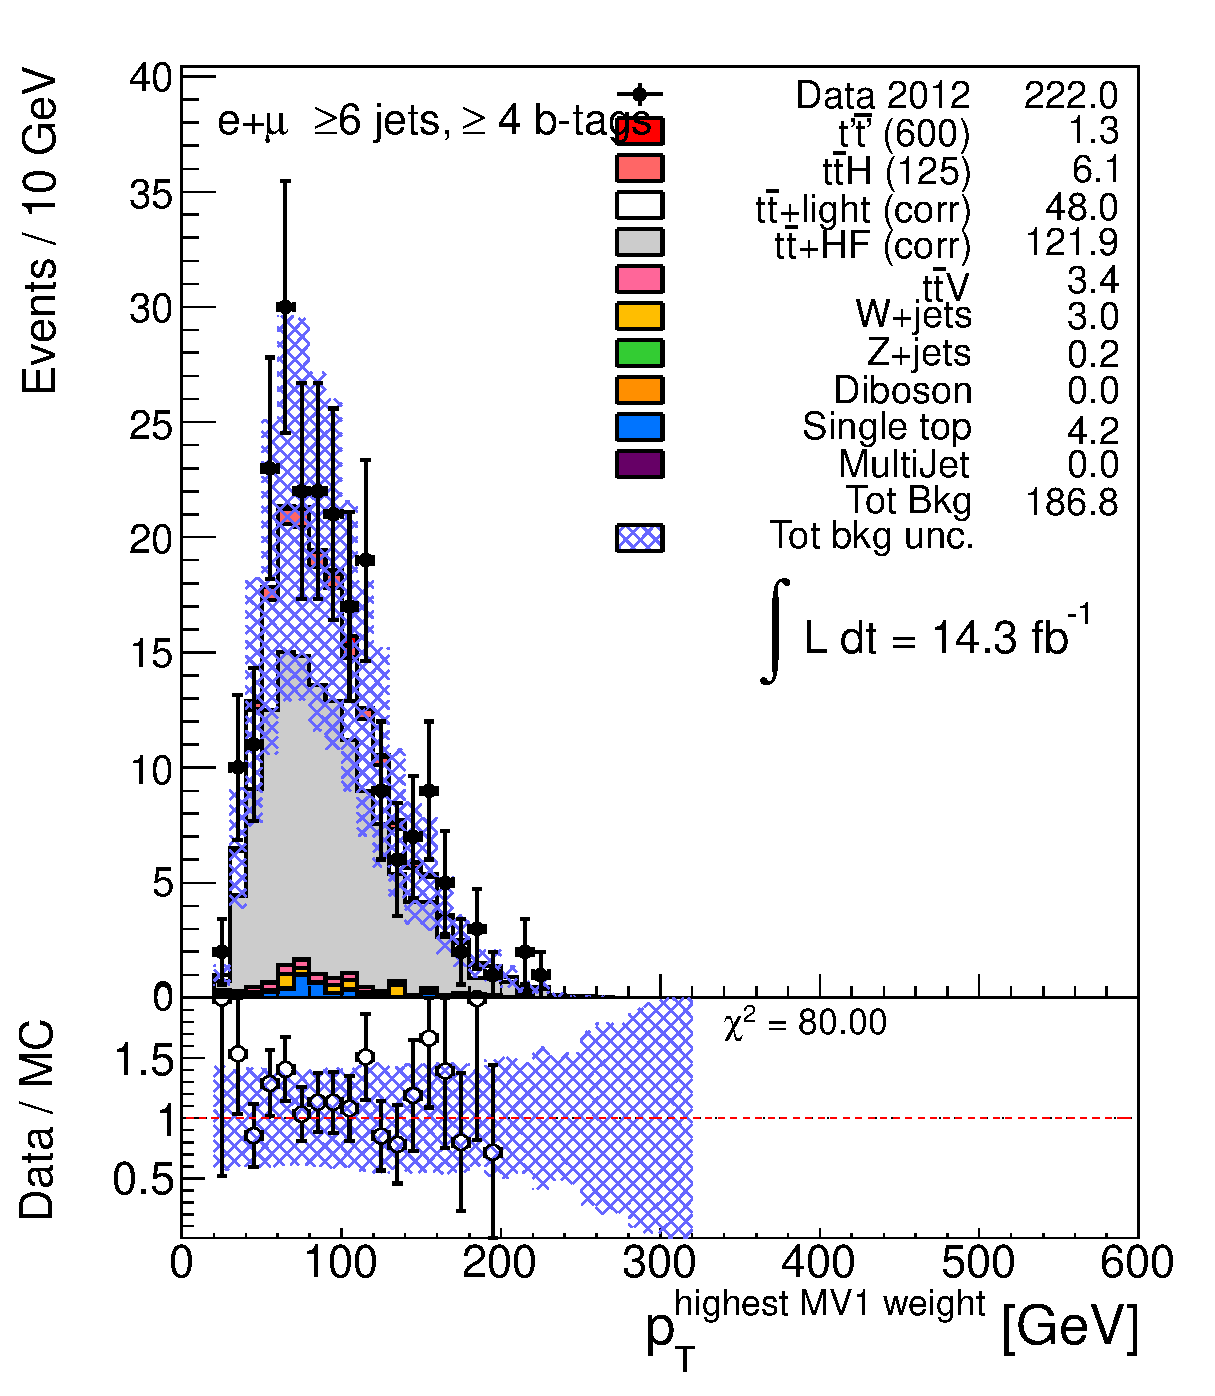
\includegraphics[width=0.235\textwidth]{htx_analysis_14ifb/figures/scaled_cr_blind/JetPtB1_ELEMUON_6jetin4btagin_NOMINAL}}
	\subfigure[]{
  	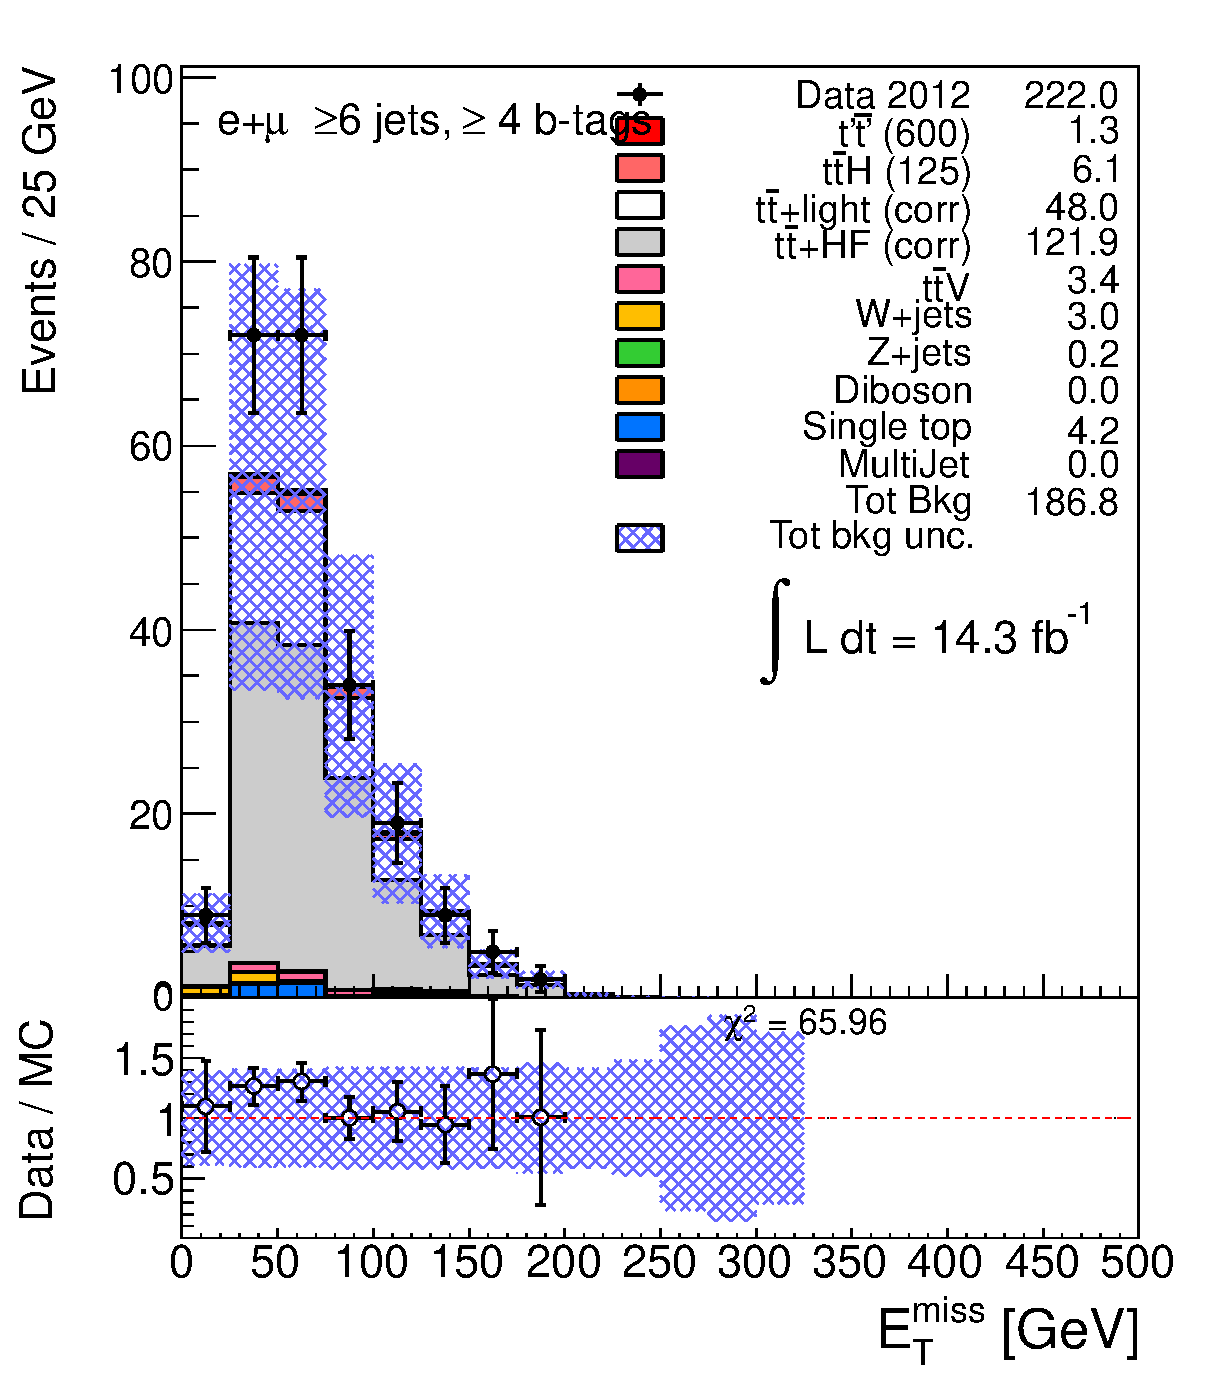
\includegraphics[width=0.235\textwidth]{htx_analysis_14ifb/figures/scaled_cr_blind/MET_ELEMUON_6jetin4btagin_NOMINAL}}
	\subfigure[]{
  	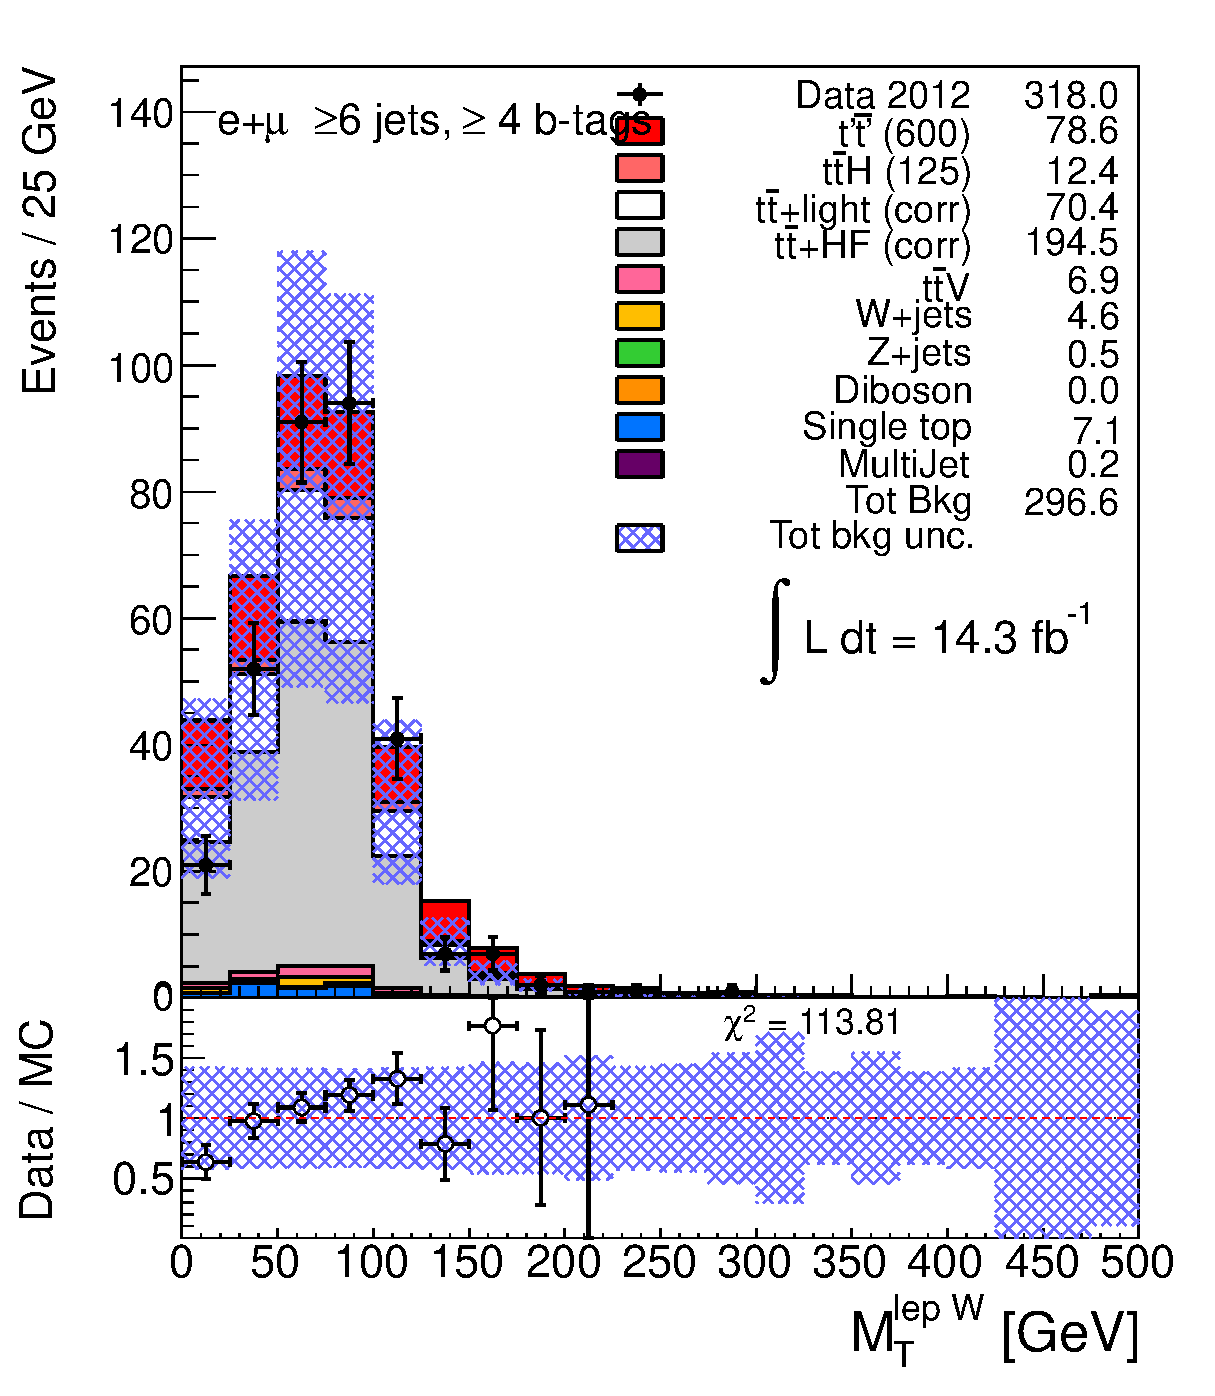
\includegraphics[width=0.235\textwidth]{htx_analysis_14ifb/figures/scaled_cr_blind/Wlep_MassT_ELEMUON_6jetin4btagin_NOMINAL}}
	\subfigure[]{
  	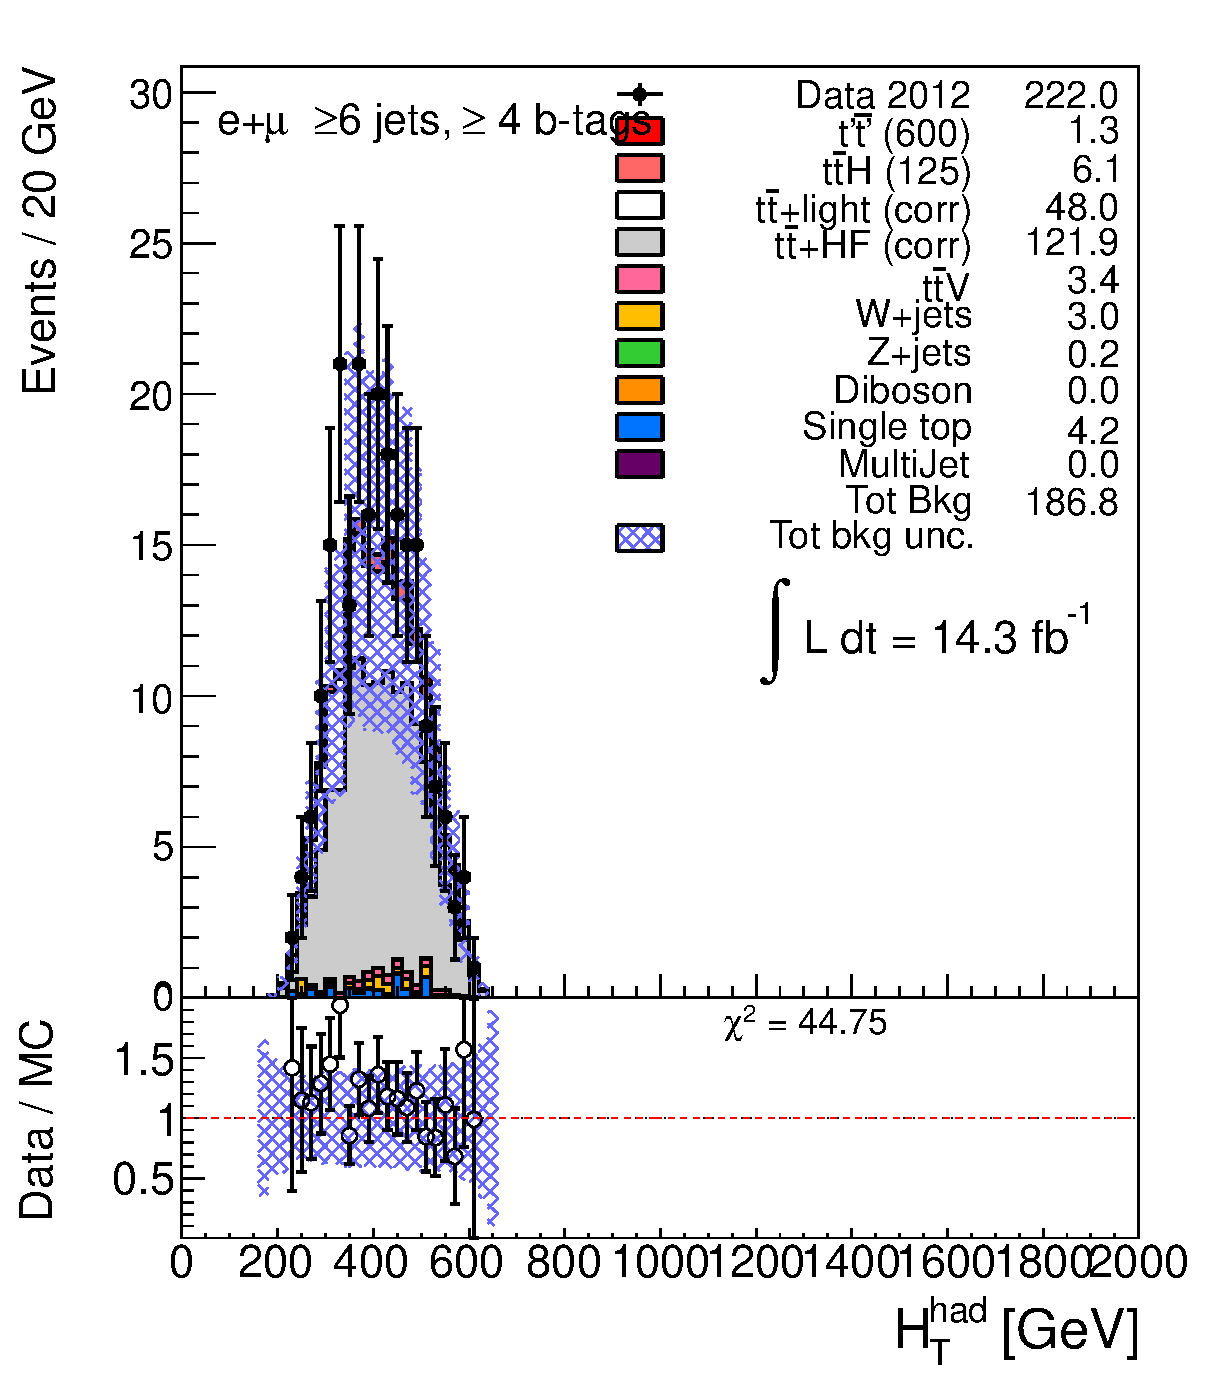
\includegraphics[width=0.235\textwidth]{htx_analysis_14ifb/figures/scaled_cr_blind/HTHad_ELEMUON_6jetin4btagin_NOMINAL}}\\
	\caption{Comparison of various distributions between data and simulation in the combined
$e$+jets and $\mu$+jets (a-d) \chii, (e-h) \chiii\ and (i-l) \chiv\ channels with 
the requirement of $\HT<700\gev$ to suppress a possible signal contribution.
The variables are, from left to right: \pt\ of the jet with the highest MV1 weight;
missing tranverse energy; transverse mass of $W$ boson; hadronic component of \HT.
The $t\bar{t}$+jets background is the nominal \texttt{ALPGEN} prediction after the fit to data (see text for details).
Also shown is the expected $\TT$ signal corresponding to $m_{\T}=600\gev$ in the $\T$ doublet scenario.
The bottom panel displays the ratio between data
and the background prediction. The shaded area represents the total background uncertainty.\label{fig:htxCRs}}
\end{center}\end{figure}

